
\documentclass[utf8]{frontiersSCNS} % for Science, Engineering and Humanities and Social Sciences articles
\usepackage[utf8]{inputenc}
%\usepackage{inputenc}
\usepackage[english]{babel}
\DeclareUnicodeCharacter{2264}{$\leq$}
\usepackage{letltxmacro}



\usepackage{stringenc}
\usepackage{pdfescape}

\makeatletter
\renewcommand*{\UTFviii@defined}[1]{%
  \ifx#1\relax
    \begingroup
      % Remove prefix "\u8:"
      \def\x##1:{}%
      % Extract Unicode char from command name
      % (utf8.def does not support surrogates)
      \edef\x{\expandafter\x\string#1}%
      \StringEncodingConvert\x\x{utf8}{utf16be}% convert to UTF-16BE
      % Hexadecimal representation
      \EdefEscapeHex\x\x
      % Enhanced error message
      \PackageError{inputenc}{Unicode\space char\space \string#1\space
                              (U+\x)\MessageBreak
                              not\space set\space up\space
                              for\space use\space with\space LaTeX}\@eha
    \endgroup
  \else\expandafter
    #1%
  \fi
}
\makeatother







\LetLtxMacro{\ORIGselectlanguage}{\selectlanguage}
\makeatletter
\DeclareRobustCommand{\selectlanguage}[1]{%
  \@ifundefined{alias@\string#1}
    {\ORIGselectlanguage{#1}}
    {\begingroup\edef\x{\endgroup
       \noexpand\ORIGselectlanguage{\@nameuse{alias@#1}}}\x}%
}
\newcommand{\definelanguagealias}[2]{%
  \@namedef{alias@#1}{#2}%
}
\makeatother

\definelanguagealias{eng}{english}
\definelanguagealias{en}{english}

\makeatletter
\let\l@eng\l@english
\makeatother

%\setcitestyle{square}
\usepackage{url,hyperref,lineno,microtype}
\usepackage[onehalfspacing]{setspace}
\linenumbers


% Leave a blank line between paragraphs instead of using \\


\def\keyFont{\fontsize{8}{11}\helveticabold }
\def\firstAuthorLast{Diego Angulo {et~al.}} %use et al only if is more than 1 author
\def\Authors{Diego Andrés Angulo\,$^{1,*}$, José Tiberio Hernández\,$^{1}$ , James Oliver and Cyril Schneider\,$^3$}
% Affiliations should be keyed to the author's name with superscript numbers and be listed as follows: Laboratory, Institute, Department, Organization, City, State abbreviation (USA, Canada, Australia), and Country (without detailed address information such as city zip codes or street names).
% If one of the authors has a change of address, list the new address below the correspondence details using a superscript symbol and use the same symbol to indicate the author in the author list.
\def\Address{$^{1}$ IMAGINE, Universidad de los Andes, Bogotá , Colombia \\
$^{2}$VRAC, Iowa State University, Ames , IA, Unites States
\\
$^{3}$AXE Neurosciences, CHUL, Quebec , QC, Canada  }
% The Corresponding Author should be marked with an asterisk
% Provide the exact contact address (this time including street name and city zip code) and email of the corresponding author
\def\corrAuthor{Diego A. Angulo}
\def\corrAddress{IMAGINE, Universidad de los Andes, Carrera 1 \# 18A -12 , Bogotá, Colombia}
\def\corrEmail{da.angulo39@uniandes.edu.co}




\begin{document}
\onecolumn
\firstpage{1}

\title[Braviz]{Braviz: Visual Exploratory Analysis of Brain Datasets} 

\author[\firstAuthorLast ]{\Authors} %This field will be automatically populated
\address{} %This field will be automatically populated
\correspondance{} %This field will be automatically populated

\extraAuth{}% If there are more than 1 corresponding author, comment this line and uncomment the next one.
%\extraAuth{corresponding Author2 \\ Laboratory X2, Institute X2, Department X2, Organization X2, Street X2, City X2 , State XX2 (only USA, Canada and Australia), Zip Code2, X2 Country X2, email2@uni2.edu}


\maketitle

%%%%%%%%%%%%%%%%%%%%%%%%%%%%%%%%%%%%%%%%%%%%%%%%%%%%%%%%%%%%%%%%%%%%%%%%%%%%%%%%%%%%%%%%%%%%%%%%%%%%%%%%%%%%%%%%%%%%%%%%%%%%%%%%%%%%%%%%%%%%%%%%%%%%%%%%%%%%%%%%%%%%%%%%%%%%%%%%%%%%%%%%%%%%%%%%%%%%%%%%%%%%%%%%%%%%%%%%%%%%%%%%%%%%%%%
%%% The sections below are for reference only.
%%%
%%% For Original Research Articles, Clinical Trial Articles, and Technology Reports the section headings should be those appropriate for your field and the research itself. It is recommended to organize your manuscript in the
%%% following sections or their equivalents for your field:
%%% Abstract, Introduction, Material and Methods, Results, and Discussion.
%%% Please note that the Material and Methods section can be placed in any of the following ways: before Results, before Discussion or after Discussion.
%%%
%%%For information about Clinical Trial Registration, please go to http://www.frontiersin.org/about/AuthorGuidelines#ClinicalTrialRegistration
%%%
%%% For Clinical Case Studies the following sections are mandatory: Abstract, Introduction, Background, Discussion, and Concluding Remarks.
%%%
%%% For all other article types there are no mandatory sections.
%%%%%%%%%%%%%%%%%%%%%%%%%%%%%%%%%%%%%%%%%%%%%%%%%%%%%%%%%%%%%%%%%%%%%%%%%%%%%%%%%%%%%%%%%%%%%%%%%%%%%%%%%%%%%%%%%%%%%%%%%%%%%%%%%%%%%%%%%%%%%%%%%%%%%%%%%%%%%%%%%%%%%%%%%%%%%%%%%%%%%%%%%%%%%%%%%%%%%%%%%%%%%%%%%%%%%%%%%%%%%%%%%%%%%%%

\begin{abstract}

%%% Leave the Abstract empty if your article falls under any of the following categories: Editorial Book Review, Commentary, Field Grand Challenge, Opinion or specialty Grand Challenge.
\section{}
Brain researchers typically deal with large amounts of data from different sources and often, of different nature. This requires the use of several different software tools and makes it cumbersome and time consuming to answer simple questions. Because of this, data is not used to its fullest potential, and exploratory analysis is rarely done . This paper presents a software tool called BRAVIZ that integrates access to several data types and automates many of the cumbersome and error-prone tasks required to explore typical neuroscience data. This work focuses on integrating interactive visualization with real-time statistical analyses to facilitate exploration and discovery. BRAVIZ enables an inversion of the typical neuroscience analysis process by emphasizing images as the main organizing objects in the process rather than relying in abstract numerical indicators. This encourages researchers to notice trends and relationships, which motivate additional analyses and generally gain a fuller understanding of the phenomena represented by the data.  A case study is presented that incorporates MRI, DTI, and fMRI images together with a large amount of neuro-psychological and clinical data.  The case study demonstrates how BRAVIZ enables researchers to discover new hypotheses about the relationships between structures and functions of the brain.

\tiny
 \keyFont{ \section{Keywords:} Exploratory Analysis, Visual Analytics, Brain Data, MRI, Tractography, Cohorts } %All article types: you may provide up to 8 keywords; at least 5 are mandatory.
\end{abstract}

\section{Introduction}

Visualizing and exploring data from brain studies is not an easy task. These studies include a large variety of data from each participant, some acquired from physical measurements or instrumentation, including neuroimages, while other information is acquired from cognitive or motor testing of the subjects. Demographical and clinical information from the subjects is also essential to make sense of the acquired data.
This work focuses on brain studies in which imaging scans are applied to a group of subjects. Several image modalities can be acquired during the scan session. This spatial data is complemented by scalar measures, and other clinical variables. Often the objective of the study is to search for differences in imaging data between groups of subjects, or to find relationships between structure and function of the brain. In such cases the mentioned context information become crucial for the analysis of the data. 


In this research, a particularly representative case study, the kmc project \cite{schneider_cerebral_2012}, is introduced to both motivate the requirements for BRAVIZ and demonstrate its effectiveness. The kmc study explores the effect of treatment options on premature births and data on subjects was collected from several fronts. The original randomized study involving about 750 preterm babies was conducted in 1994 \citep{charpak_kangaroo_1997}. These kids were followed during their first year \citep{charpak_randomized_2001, tessier_kangaroo_2009} of life and several clinical and socio-economical variables were registered. Forty of the kids from the original study were re located at fifteen years of age, the  subjects went through several neuro-psychological tests, measuring attention, memory, reasoning skills and hand-eye coordination among others. They also went to vision, hearing and full medical examinations. Finally, they were scanned with Structural MRI, DTI and several fMRI protocols. \footnote{agregar este protocolo} These images were processed using freesurfer \citep{fischl_freesurfer_2012}, fsl\citep{jenkinson_fsl_2012}, camino\citep{cook_camino:_2006}, and spm\citep{friston_statistical_2006}; which extracted several numerical measurements and geometric structures as segmentations and tractographies. All of this data was collected for testing specific hypotheses but the specialists involved in the study are also interested in analyzing it for unexpected relationships and trends; in other words, to perform an exploratory analysis\citep{tukey_we_1980}.


Exploratory analyses require visualizing different kinds of data, and interactively moving through it, and across participants. It requires visualizing image data in context; and tracing numerical features back to the image of origin. It is necessary to have an overview of the data in order to grasp patterns and detect outliers. Outliers need to be analyzed closely to understand if they are real data or the result of some mistake (see \cite{schneiderman_designing_1998}). 

Current analysis tools  are designed to support the different steps of confirmatory analysis, and most image viewers are designed for quality control or for producing publication level images. However, exploratory research requires integrated analysis and visualization tools that provide immediate access to the data. Confirmatory analysis is a careful linear process, which starts with a hypothesis, processes data in a specific manner and performs planned statistics in order to prove the hypothesis. In contrast exploratory analysis is iterative and goes through the data multiple times in different ways. The objective is to find trends, patterns and general insights in the data, which may later become hypotheses that can be tested in a new experiment.

Visual analytics\citep{cook_illuminating_2005} is a emerging field that attempts to put human experts and machines at the same level so that, working together, data can be better understood. This requires very efficient communication between the computer and the expert, which is accomplished through rich interactive visualizations. In visual analytics the strengths of computers and human experts complement each other. Human creativity, intuition, and expertise can guide the analysis into unexpected areas. Applying the visual analytics framework to neuroscience will allow researchers to extract more information from their large, multi-source and labor-intensive datasets, and potentially lead to new discoveries.

This paper presents BRAVIZ, a software tool to facilitate visual exploration of brain data. It provides access to image data such as MRI, fMRI and DWI, as well as processed data, like surface segmentations, activation volumes and tractographies. It also supports access to tabular data and integrates some simple statistical analysis tools. In contrast to the conventional workflow that introduces visualization only at the end of the analysis, BRAVIZ positions interactive visualization at the core of exploratory research. Simple, efficient and intuitive access to visualization facilitates creation of analysis input, evaluation of analysis results, and inspiration of new research hypotheses. The system was designed following a user-centered methodology and aims to solve the bottlenecks identified in neuroscience domain experts’ workflow. To maintain interactivity and provide high quality analysis tools, BRAVIZ leverages several state state-of-the-art open-source applications and libraries.  The contributions of the systems can be summarized as:
\begin{itemize}
\item Visualization integrated at every step
\item "Details on demand" via integrated data linking 
\item Accelerated exploratory research by removing data access overhead
\item Support concrete domain user needs
\item Give researchers access to data that is typically out of their area of expertise, and improve communication between experts
\item Opportunistic integration of existing tools and algorithms.

\end{itemize}

%\begin{methods}
\section{Description}

BRAVIZ was designed following a "user centered" approach\citep{fernandez_user-centered_2013,wassink_applying_2009}. The authors worked closely with brain researchers of several specialties, visited several labs and hospitals, and learned as much as possible about typical neuroscience research workflows. An extensive literature review in the domain led to better understanding of the kinds of data patterns neuroscience researchers find interesting. In addition, the graphics and pictures in these publications were used as models for BRAVIZ visualizations so that they would look familiar to the neuroscience research community. The design, development and evaluation process consisted of several iterative cycles, prototypes were shared with domain experts, and their feedback motivated design ideas and usability enhancements for the next generation. As the development cycles progressed, the domain experts ventured further away from common paradigms; they were encouraged to dream, and not to worry about how complex it would be to implement the ideas. 

Instead of one large application with numerous features and controls, BRAVIZ is divided into several small tools. Individual tools are tailored towards specific tasks and therefore are easy to learn and use. This tools are designed to analyze cohort data, i.e., data that is composed from a set of subjects with several measures. Smaller samples of subjects, or subsamples, can also be analyzed and compared against each other. Nominal or numerical measures of the subjects are called variables, and these complement the neuro-image based spatial data. Note that the set of variables can be extended by deriving new values from spatial data or existing variables. 

BRAVIZ tools combine numerical and nominal variables with spatial data. There are tools to look at spatial data from a single subject with high detail, as well as tools to look at spatial data associated with a subsample; both with numerical and categorical data as context. Another group of tools is focused on exploring these variables, but always linking back to details of each subject.

Each of the tools has data visualization as its centerpiece. This visualization can be customized, usually by adding or removing variables or spatial data, according to the question at hand. The state of the visualization can be saved  to recall it at a future time or to share it with colleagues. 

All visualizations are interactive and capable of generating a dialogue with the user.
As Colin Ware \citep{ware_information_2004} said "The best visualizations are not static images to be printed in books, but fluid, dynamic artefacts that respond to the need for different views or for more detailed information".  

Though the system is built from several small applications, they are designed to work together synchronously in order to support more complex tasks. Subsamples, variables and subjects of interest can be shared across tools and among colleagues. 
Several of the calculations are made ahead of time and kept in a cache in order to speed-up response at analysis time. These features, combined with having all data and analysis tools a couple of clicks away; provides a pleasant and efficient exploratory analysis environment. 

A main objective of the project is fostering collaboration between experts, especially inside teams including multiple specialties. Thus the initial stages of design focused on identifying the obstacles that affected communication between experts, and looked explored ways of mitigating them. The team of experts was composed of radiologists, psychiatrists, pediatricians, physicians, physiologists, statisticians, engineers and economists. Each of these groups of experts typically utilizes tools designed to foster their analysis and contribution to the team, but very few develop skills in tools outside of their areas of expertise.

For example, several experts in neuroimaging typically use Freesurfer  \citep{fischl_freesurfer_2012}, fsl\citep{jenkinson_fsl_2012} and spm \citep{friston_statistical_2006} toolkits to analyze data. All of these sets include applications for interactive visualization. 3D slicer \citep{fedorov_3d_2012}, Brain Visa \citep{cointepas_brainvisa:_2001} and ITKSnap \citep{yushkevich_user-guided_2006} are other commonly used tool which provide advanced visualization and processing features. On the clinical side Osirix\citep{rosset_osirix:_2004} and proprietary software bundled with PACS and imaging equipment are very popular. By analyzing these tools, and the way  experts use them, the BRAVIZ team learned what was expected from image viewers, which features were important and which ones were seldom used. This effort also exposed typical process bottlenecks that affect efficient exploratory analyzes.

In statistics, data exploration tools like ggobi\citep{cook_interactive_2007}, aabel, SPSS, stata and Tableau\citep{hanrahan_tableau_2003} are used to analyze and explore datasets. Using these tools it is possible to transform data, fit models, and visualize relationships.  Interactive visualizations let the user explore complex relationships in the data, detect outliers and interesting subgroups, and grasp subtle patterns and trends. These tools implement techniques such as brushing, zooming and point identification. Insights discovered in this way can be used to develop hypotheses and tested in further experiments. 

In a typical neuroscience research group, both types of tools (visualization and statistical analysis) complement each other, and it is common for experts to use them at the same time. However moving data from one side to the other  is not trivial. While most statistical tools implement interactions that allow the user to iterate very efficiently through the data, the process for creating visualizations in the neuroimage side requires significant work; and is often focused on a single subject. Most of these tools were designed for classical hypothesis testing or case studies, and are very good for this purpose. The goal of BRAVIZ is to provide a tool that integrates the best of both worlds and better supports exploratory analyzes with spatial data. A crucial aspect is providing a direct bridge between statistics and neuroimage visualizations. By integrating concepts from both worlds BRAVIZ seeks to grasp the attention of all kinds of specialties and increase communication between them. 

%Include also here the not repeated paragraphs from the Methodology (really motivation) section of the last draft.


\subsection{BRAVIZ Tools}

%Not sure if this needs a different section, maybe it should be summarized into the description

The current set of applications comprising BRAVIZ can be divided in three categories. One set of applications focuses on displaying geometric data using other variables as context, another focuses on manual measuring or creating new descriptors from geometric data, ant the last one focuses on exploring numerical and categorical data while maintaining a link to the underlying geometric data. Additionally there are tools for importing and exporting data in spreadsheet format; so that the tools can interact with statistical software. All tools are accessible from a graphical menu as shown in figure \ref{fig_menu}. The tools included in the current version are

\begin{itemize}
\item Create and Measure: Define new scalars of geometric structures based on spatial data for the whole cohort.
\begin{itemize}
\item Roi Builder: Create spherical regions of interest, using images or surfaces as context.
\item Linear Measure: Measure elements of any image using lines
\item Logic Bundles: Define fiber bundles by doing logical operations on ROIs and segmented structures.
\end{itemize}
\item Visualize Spatial Data: Explore different kinds of spatial data in context.
\begin{itemize}
\item Subject Overview: Visualize several spatial objects, as well as context information for a single subject.
\item Sample Overview: Repeat the same visualization for a group of subjects, sorted by a numerical variable and divided in groups by a nominal variable.
\item Explore fMRI: Visualize BOLD timelines, experiment design and contrasts (read from spm file).
\item Check Registration: Visualize two images at the same time to evaluate the quality of registration. 
\end{itemize}
\item Analysis: Analyze data from tables together with variables derived from spatial data. 
\begin{itemize}
\item Anova : Perform ANOVA analyzes on the database variables,
\item Linear Model: Fit a Linear model to variables in the database.
\item Correlations: Explore correlations between variables in the database.
\item Parallel Coordinates: Visualize multiple variables in interactive parallel coordinates.
\end{itemize}
\end{itemize} 

The main interface of the Subject Viewer application is shown on figure \ref{fig_subject}. This tool provides access to MRI Images, Freesurfer semgentations and reconstruction, tractographies, tracula bundles and fMRI maps; all through graphical menus. The user never needs to know which files are involved in displaying a particular scene. Some geometrical features, as volume or mean FA inside a structure, can be captured directly from  this application and added into the database as a new variable. 

Below the main view (as shown in Figure \ref{fig_subject}) is a context panel, that displays the values of selected variables for the current subject. To change the current subject the user may use the controls underneath the main view, or select from the table in the subjects panel at the left. All of the current selected variables and geometric objects in the view are updated to display the information for the new subject. Thus it is straightforward to look at a certain aspect across different subjects. In the lower left corner is a control that allows the user to select between native MRI coordinate systems, Talairach space or Dartel template space (involves non linear registration). All of the geometric objects in the scene are shown in the selected coordinate space. The Talairach and Dartel spaces make it easy to compare among different subjects but may add some distortion to the objects, so the user must pick the most appropriate coordinates for the task at hand. 

A small-multiples view[19] display of several subjects, as shown in figure \ref{fig_sample}, is available in the sample overview application. This application is useful for finding trends across a sample or doing quality control and spotting problematic images. Subjects are arranged from left to right according to a numerical variable, and rows are defined by a nominal variable. In the example shown the two rows are males and females, and the ordering variable is the score in a math test. The bar-plot at the right shows the distribution of the variable among the two groups and is coordinated with the 3d views.A bar-plot is used because it provides the best sense of magnitude differences for variables that have a meaningful zero. Each view shows a collection of objects defined in the subject overview application. In this way the interface is kept simple, as there is no need for visual configuration options.

As before different coordinates systems can be used to make comparisons easier. The camera between the small multiples is also coordinated, if the view is changed in any of the views, the others are changed accordingly. In addition if the user is interested in getting a more detailed view of any of them, he can right click and from the context menu open a full subject viewer application with the correct scenario and subject loaded, or make all opened BRAVIZ applications switch to the corresponding subject.

At the core of BRAVIZ is a database that contains clinical and demographic data, as well as results from neuropsychological tests or questionnaires; and enriched with geometric indicators generated in external tools or inside BRAVIZ. All of the individual tools that BRAVIZ provides are integrated with the database. BRAVIZ provides several common statistical analysis tools that access this database, as for example, an ANOVA  analysis, which can be completed with the application shown in figure \ref{fig_anova}. In order to perform the analysis the user must select an outcome variable, one or more regressors and optionally interaction terms. It is also possible to limit the analysis to a specific subset of subjects. Afterwards it is only necessary to click on the Calculate Anova button, which fetchs the required data from the database and performs the calculation\footnote{Maybe there is no need to mention R here}. The main plot will initially show diagnostics, i.e. distribution of residuals and a scatter plot of residuals vs fitted values. The table at the bottom right shows the resulting fitted values. By double clicking on any row a plot showing the effect of that particular term will be displayed. From this plot it is possible to right click on an outlier to get additional information, or to show him on any other opened BRAVIZ applications. This plot will also respond to messages from other applications and highlight the corresponding subject.

It is worth noting that no correction for multiple comparisons is applied in the statistical tests; so care must be taken when interpreting the results. The objective here is not to prove hypotheses but to explore data and find interesting hypotheses, which should be tested using the usual methods.

Figure \ref{fig_other_apps} shows several other applications currently built into the system. More information as well as the source code for the project can be found at http://diego0020.github.io/braviz


\section{Related Work}

In recent years the amount of MRI-Data collected has grown significantly. It is also increasingly common to find large medical image databases open for analysis, such as the human connectome project\citep{rosen_human_2010} and ADNI\citep{jack_alzheimers_2008}. This has created a need for exploration tools that will allow researchers from around the world to extract knowledge from this data. Notice that the interest here shifts from hypothesis testing towards hypothesis generation, and therefore the workflow is completely different.
  
INVIZIAN\citep{bowman_query-based_2011,bowman_feature-similarity_2012} is an application for exploring large brain datasets which integrates structural and scalar data. It organizes data in an abstract 3D space in such a way that similar brains are located close to one another. The system can display more or fewer details of each brain depending on the zoom level. It is also integrated with gGobi\citep{cook_interactive_2007} in order to explore relations between scalar values and more complex brain features. It can handle datasets of several hundreds of brains and it uses sophisticated data mining algorithms, feature extraction and abstract spaces to create the representation. The main different to our approach is that BRAVIZ focuses on leveraging the creativity, intuition, experience and knowledge of the human expert while INVIZIAN focuses on machine learning methods. In the future both approaches should be integrated.

The Visual Analytics of Brain Networks\citep{li_visual_2012} (VABN) software is focused on analyzing large connectivity datasets by defining a robust and repeatable algorithm for region of interest (ROI) placement that will act as nodes. This creates comparable networks that can be analyzed with graph based methods. The tool provides access to the underlying DWI or fMRI data in order to initially place the ROIs and to verify the results. The methods and software libraries used in this tool are very similar to BRAVIZ. However the objectives of both projects are different, as VABN does not seek to integrate connectivity data with other kinds of data. In the future VABN’s network analyzes could be integrated into BRAVIZ to further extend its capabilities.

\section{Implementation}

BRAVIZ implemented in Python which is now popular in the neuroscience community \citep{gorgolewski_nipype:_2011, garyfallidis_dipy_2014}.  Powerful plotting, rendering, and data manipulation libraries are available, and because it is an interpreted language it can be used interactively and debugging is simpler. The trade-off is a loss of performance compared to compiled languages, but so far interactivity has been maintained by letting VTK\citep{schroeder_vtk_1998} and Numpy\citep{van_der_walt_numpy_2011} do the most expensive operations. It has been tested in Mac, Windows and Linux.

Mechanisms to read and display several kinds of spatial data are implemented, including images, freesurfer \citep{fischl_freesurfer_2012} cortex reconstructions and tractographies. This information is integrated with variables which can be stored as numerical values or labels. These can be derived from geometric objects by, for example, averaging FA over a region, by measuring the volume of a segmented structure, defining new fiber bundles and measuring their mean FA or by measuring the length of a given structure. These variables can then be used in the same way as the original context variables.

BRAVIZ is also a library that can be used for creating custom visualizations to support specific tasks. Figure \ref{fig_arch} shows the general architecture.

The "Read and Filter" module handles all access to the file system or network. Each BRAVIZ project is composed of a SQLite database, and the images and other geometric data. Specific project reader modules can be created to adjust to the layout, file names and other peculiarities of each project. The active project, favorite variables and favorite subject, are specified through a configuration file. This module provides other useful functions like attaching scalars to geometric objects, filtering fiber bundles and transforming between coordinate systems. Underneath it relies heavily on nibabel\citep{gorgolewski_nipype:_2011}, numpy\citep{van_der_walt_numpy_2011} , scipy\citep{jones_$$scipy$$:_2014} and VTK\citep{schroeder_vtk_1998} . Notice that this module handles all the necessary transformations of spatial data, and exposes a high level interface to the upper layers. In this way application designers can focus on visualization and interaction as required by end users and let the library handle registration and other low level operations. Accessing data through this module, allows developer to create applications that can be easily ported to different projects. 

The "Read and filter" module also provides access to numerical and categorical variables that are stored in a SQLite database. Pandas' DataFrames\citep{mckinney_data_2010} are the preferred way to manipulate data and move it through the different components of an application. This database also holds annotations, scenarios, and user defined geometrical objects. 

The "visualization" module provides reusable components for visualizing 3D geometric data and scalar data. VTK is used for all the 3D visualization while 2D visualization is achieved through matplotlib \citep{hunter_matplotlib:_2007} and seaborn\citep{michael_waskom_seaborn:_2014}.

The "interaction" modules contains, among others, several reusable user interface components, and functions for doing statistical calculations in R\citep{team_r:_2012} through the rpy2 \citep{gautier_rpy2:_2008} python package. The current version uses PyQt4 for the user interface with some web based visualizations built using the tornado\citep{server_source_2008} framework  This module also contains code to handle communication between different applications through the 0mq protocol\citep{hintjens_zeromq:_2013}.

\section{Case Study}

\section{Discussion}

Future work
Web based?
\section{Figures}

\section*{Acknowledgments}


\bibliographystyle{frontiersinSCNS_ENG_HUMS} % for Science, Engineering and Humanities and Social Sciences articles, for Humanities and Social Sciences articles please include page numbers in the in-text citations
%\bibliographystyle{frontiersinHLTH&FPHY} % for Health and Physics articles
\bibliography{zotero}

%%% Upload the *bib file along with the *tex file and PDF on submission if the bibliography is not in the main *tex file

\section*{Figures}

%%% Use this if adding the figures directly in the mansucript, if so, please remember to also upload the files when submitting your article
%%% There is no need for adding the file termination, as long as you indicate where the file is saved. In the examples below the files (logo1.jpg and logo2.eps) are in the Frontiers LaTeX folder
%%% If using *.tif files convert them to .jpg or .png
\begin{figure}[h!]
\begin{center}
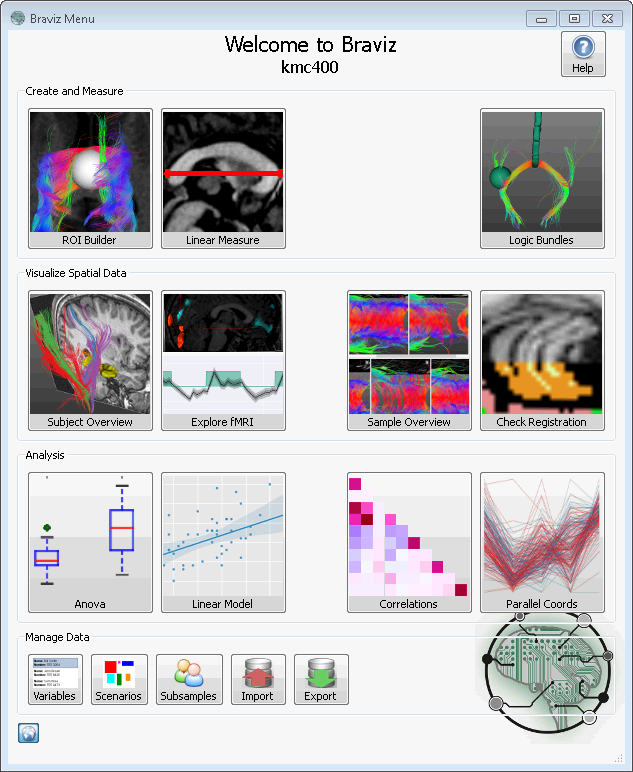
\includegraphics[width=0.4\textwidth]{figures/braviz_menu.PNG}
\end{center}
 \textbf{\refstepcounter{figure}\label{fig_menu} Figure \arabic{figure}.}{This menu is currently used to access the different applications. It also provides facilities to review the available variables and the saved scenarios, to view and create subsamples, and to import to and export from spreadsheets.  }
\end{figure}

\begin{figure}[h!]
\begin{center}
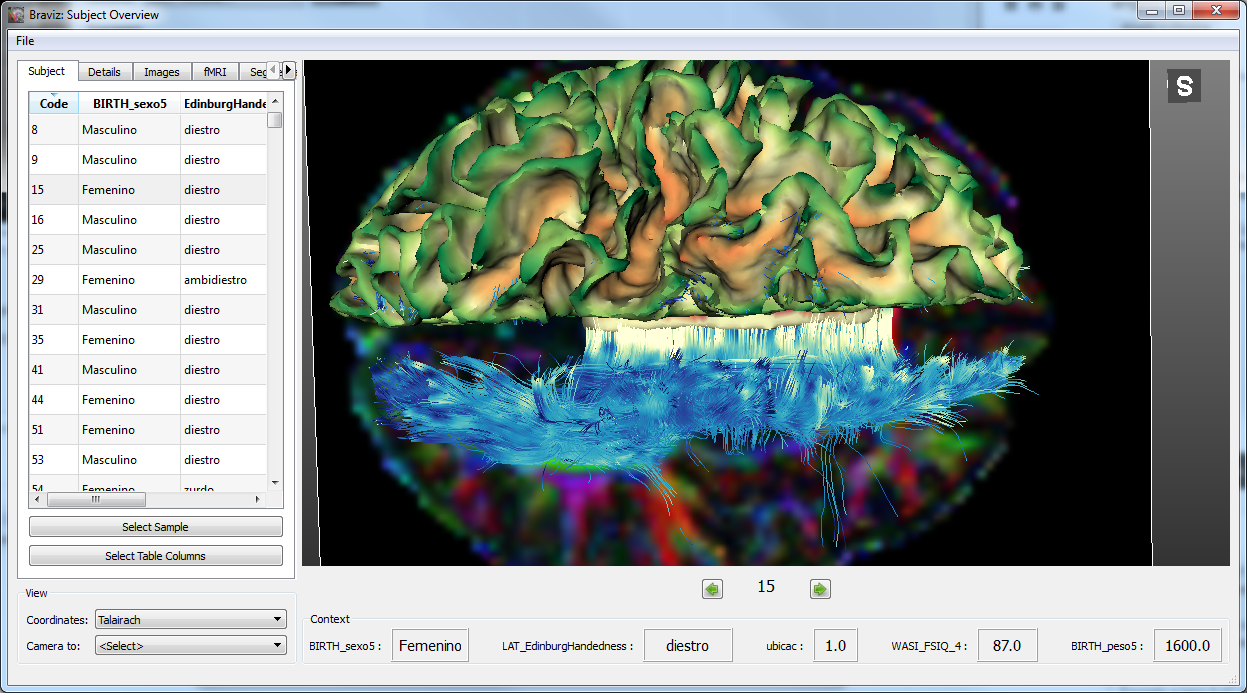
\includegraphics[width=0.9\textwidth]{figures/subj_overview_full.PNG}
\end{center}
 \textbf{\refstepcounter{figure}\label{fig_subject} Figure \arabic{figure}.}{Main interface of the subject overview application. At the bottom of the render panel some variables about the subject are shown to provide context. At the bottom-left corner we have controls to change the coordinate system, and to move the camera to preset positions. Most of the data is available via the different tabs at the left panel. The current tab provides a list of available subjects, it is enough to double click in a row to get the selected data for that subject. The arrows directly under the 3d viewer provide another convenient way to move through the subjects following the order of the list. }
\end{figure}

\begin{figure}[h!]
\begin{center}
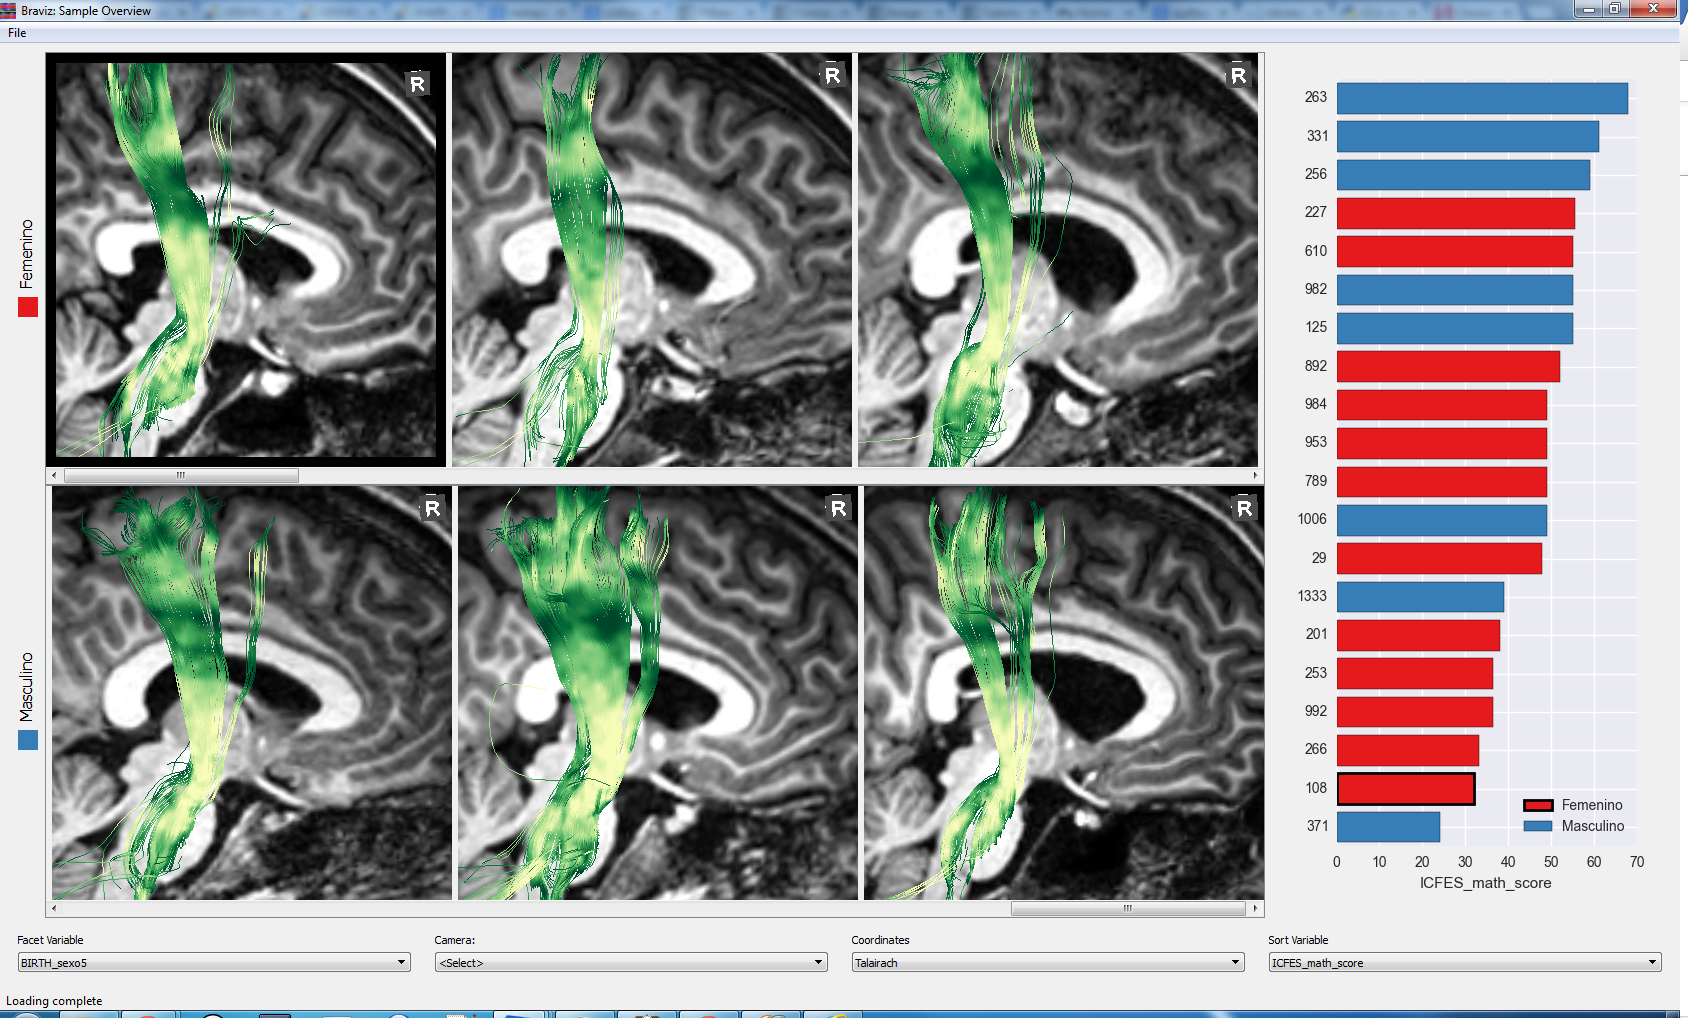
\includegraphics[width=0.9\textwidth]{figures/sample_overview.PNG}
\end{center}
 \textbf{\refstepcounter{figure}\label{fig_sample} Figure \arabic{figure}.}{This application gives access to the data of several subjects at the same time. Images are sorted from left to right according to a numerical variable (shown in the bars at the right) and arranged in columns by a cathegorical variable (bars color)  }
\end{figure}

\begin{figure}[h!]
\begin{center}
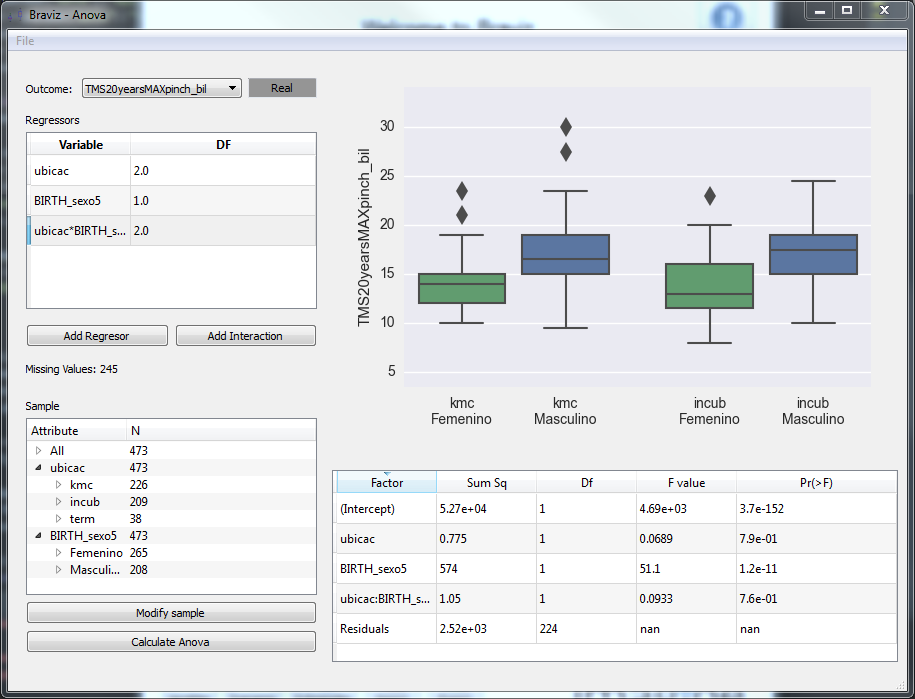
\includegraphics[width=0.9\textwidth]{figures/anova.PNG}
\end{center}
 \textbf{\refstepcounter{figure}\label{fig_anova} Figure \arabic{figure}.}{An application for performing ANOVA analyses using the data in the BRAVIZ database. You can right click on an outlier to select it on all open BRAVIZ applications. }
\end{figure}

\begin{figure}[h!]
\begin{center}
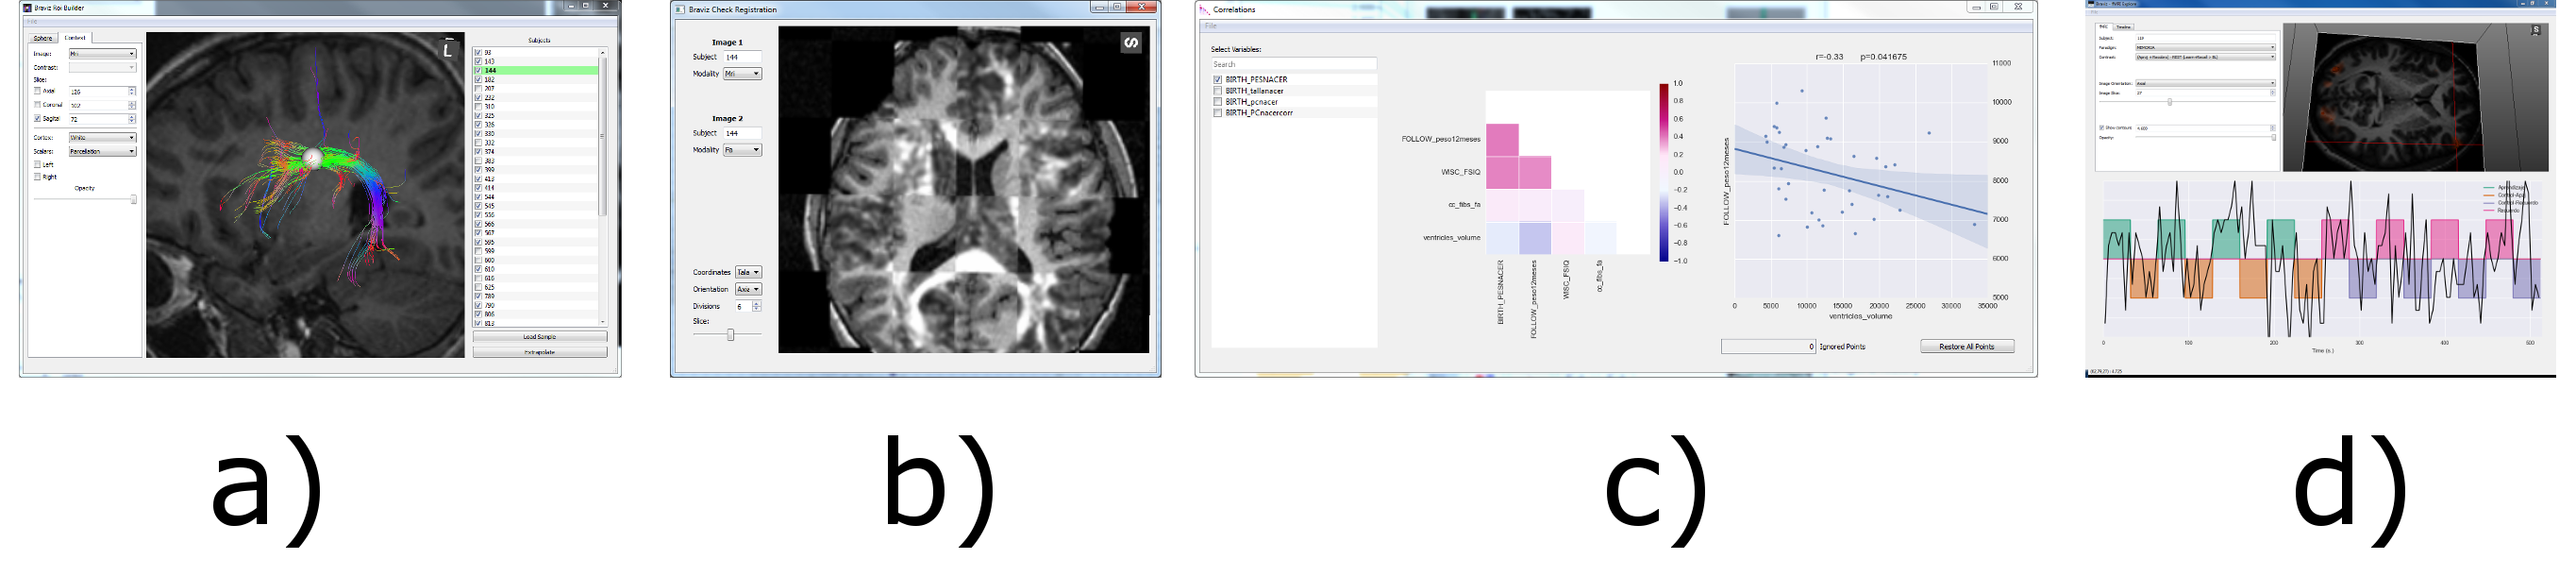
\includegraphics[width=0.9\textwidth]{figures/many_apps.png}
\end{center}
 \textbf{\refstepcounter{figure}\label{fig_other_apps} Figure \arabic{figure}.}{Examples of currently available applications. A) ROI builder. B) Linear model. C) Explore fMRI. D) Correlations. E) Parallel coordinates}
\end{figure}

\begin{figure}[h!]
\begin{center}
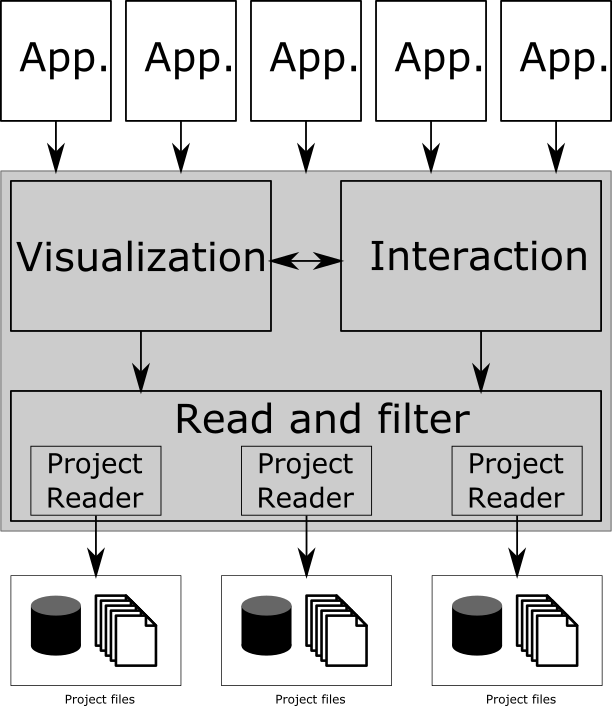
\includegraphics[width=0.9\textwidth]{figures/arquitecture.png}
\end{center}
 \textbf{\refstepcounter{figure}\label{fig_arch} Figure \arabic{figure}.}{The BRAVIZ software architecture. At the bottom there are specialized reader classes for each data-set which handles low level access to the specific projects' data. In gray is the main  library, which provides modules for visualization, interaction and data manipulation. On top user applications are built. In order to adapt the system to a new data-set it is only necessary to adapt a project reader.}
\end{figure}

\end{document}
